\documentclass[compress]{beamer}
\usepackage{ifthen,verbatim}

\newcommand{\isnote}{}
\xdefinecolor{lightyellow}{rgb}{1.,1.,0.25}
\xdefinecolor{darkblue}{rgb}{0.1,0.1,0.7}

%% Uncomment this to get annotations
%% \def\notes{\addtocounter{page}{-1}
%%            \renewcommand{\isnote}{*}
%% 	   \beamertemplateshadingbackground{lightyellow}{white}
%%            \begin{frame}
%%            \frametitle{Notes for the previous page (page \insertpagenumber)}
%%            \itemize}
%% \def\endnotes{\enditemize
%% 	      \end{frame}
%%               \beamertemplateshadingbackground{white}{white}
%%               \renewcommand{\isnote}{}}

%% Uncomment this to not get annotations
\def\notes{\comment}
\def\endnotes{\endcomment}

\setbeamertemplate{navigation symbols}{}
\setbeamertemplate{headline}{\mbox{ } \hfill
\begin{minipage}{5.5 cm}
\vspace{-0.75 cm} \small
\end{minipage} \hfill
\begin{minipage}{4.5 cm}
\vspace{-0.75 cm} \small
\begin{flushright}
\ifthenelse{\equal{\insertpagenumber}{1}}{}{Jim Pivarski \hspace{0.2 cm} \insertpagenumber\isnote/\pageref{numpages}}
\end{flushright}
\end{minipage}\mbox{\hspace{0.2 cm}}\includegraphics[height=1 cm]{../cmslogo} \hspace{0.1 cm} \includegraphics[height=1 cm]{../tamulogo} \hspace{0.01 cm} \vspace{-1.05 cm}}

\begin{document}
\begin{frame}
\vfill
\begin{center}
\textcolor{darkblue}{\Large Tracker weak mode update}

\vfill
\begin{columns}
\column{0.3\linewidth}
\begin{center}
\large
\textcolor{darkblue}{Jim Pivarski}
\end{center}
\end{columns}

\begin{columns}
\column{0.3\linewidth}
\begin{center}
\scriptsize
{\it Texas A\&M University}
\end{center}
\end{columns}

\vfill
 1 March, 2010

\end{center}
\end{frame}

%% \begin{notes}
%% \item This is the annotated version of my talk.
%% \item If you want the version that I am presenting, download the one
%% labeled ``slides'' on Indico (or just ignore these yellow pages).
%% \item The annotated version is provided for extra detail and a written
%% record of comments that I intend to make orally.
%% \item Yellow notes refer to the content on the {\it previous} page.
%% \item All other slides are identical for the two versions.
%% \end{notes}

\small

\begin{frame}
\frametitle{News}
\begin{itemize}\setlength{\itemsep}{0.5 cm}
\item I implemented a general module for making residuals vs.\ track
  curvature plots for all first-station chambers (and in relevant
  groups) in Alignment/CommonAlignmentMonitor
\item These are for monitoring the tracker tracks that we get for
  alignment, to see if there is any inconsistency in them (there
  currently is)
\item I've made some exploratory plots with the new package, and will
  be integrating this into CVS soon, then will add a twiki for
  long-term reference
\item This should also be merged into Vadim's plotter, with a
  medium-term priority
\end{itemize}
%% \hspace{-0.83 cm} \textcolor{darkblue}{\Large Outline2}
\end{frame}

%% \section*{First section}
%% \begin{frame}
%% \begin{center}
%% \Huge \textcolor{blue}{First section}
%% \end{center}
%% \end{frame}

\begin{frame}
\frametitle{Example plot (with annotations)}
\begin{itemize}
\item The $A + B \exp(-x^2/2/0.01^2)$ fit (red) is empirical, but fits all chambers well (100~GeV/c is special, probably tracker radius)
\item There's a plot like this for all DT wheels, all sectors of station~1
\item Similar plot for every CSC in ME1/1, 1/2, 1/3 (all 36 chambers),
  also grouped into pseudo-sectors (12 groups of 3 chambers, roughly
  aligned with barrel's sectors), and all-evens, all-odds
\end{itemize}

\vfill
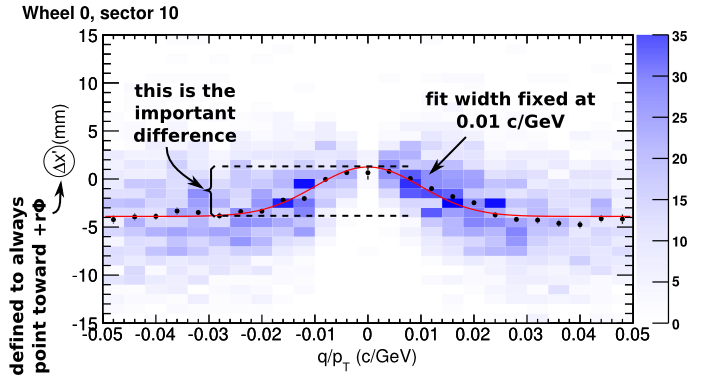
\includegraphics[width=0.8\linewidth]{example.png}
\end{frame}

\begin{frame}
\frametitle{Another way to look at it}

\begin{itemize}
\item By taking numerical derivatives with the propagator, we can
  compute the track momentum bias (assuming the chamber is well-aligned)
\item Even if the chamber is not properly aligned, it gives a sense of
  the scale of momentum errors (in another study, varying chamber
  alignment just changes the lineshape, but not the typical scale)
\item This is also in the set of plots, along with curvature bias $\Delta (q/p_T)$
\end{itemize}

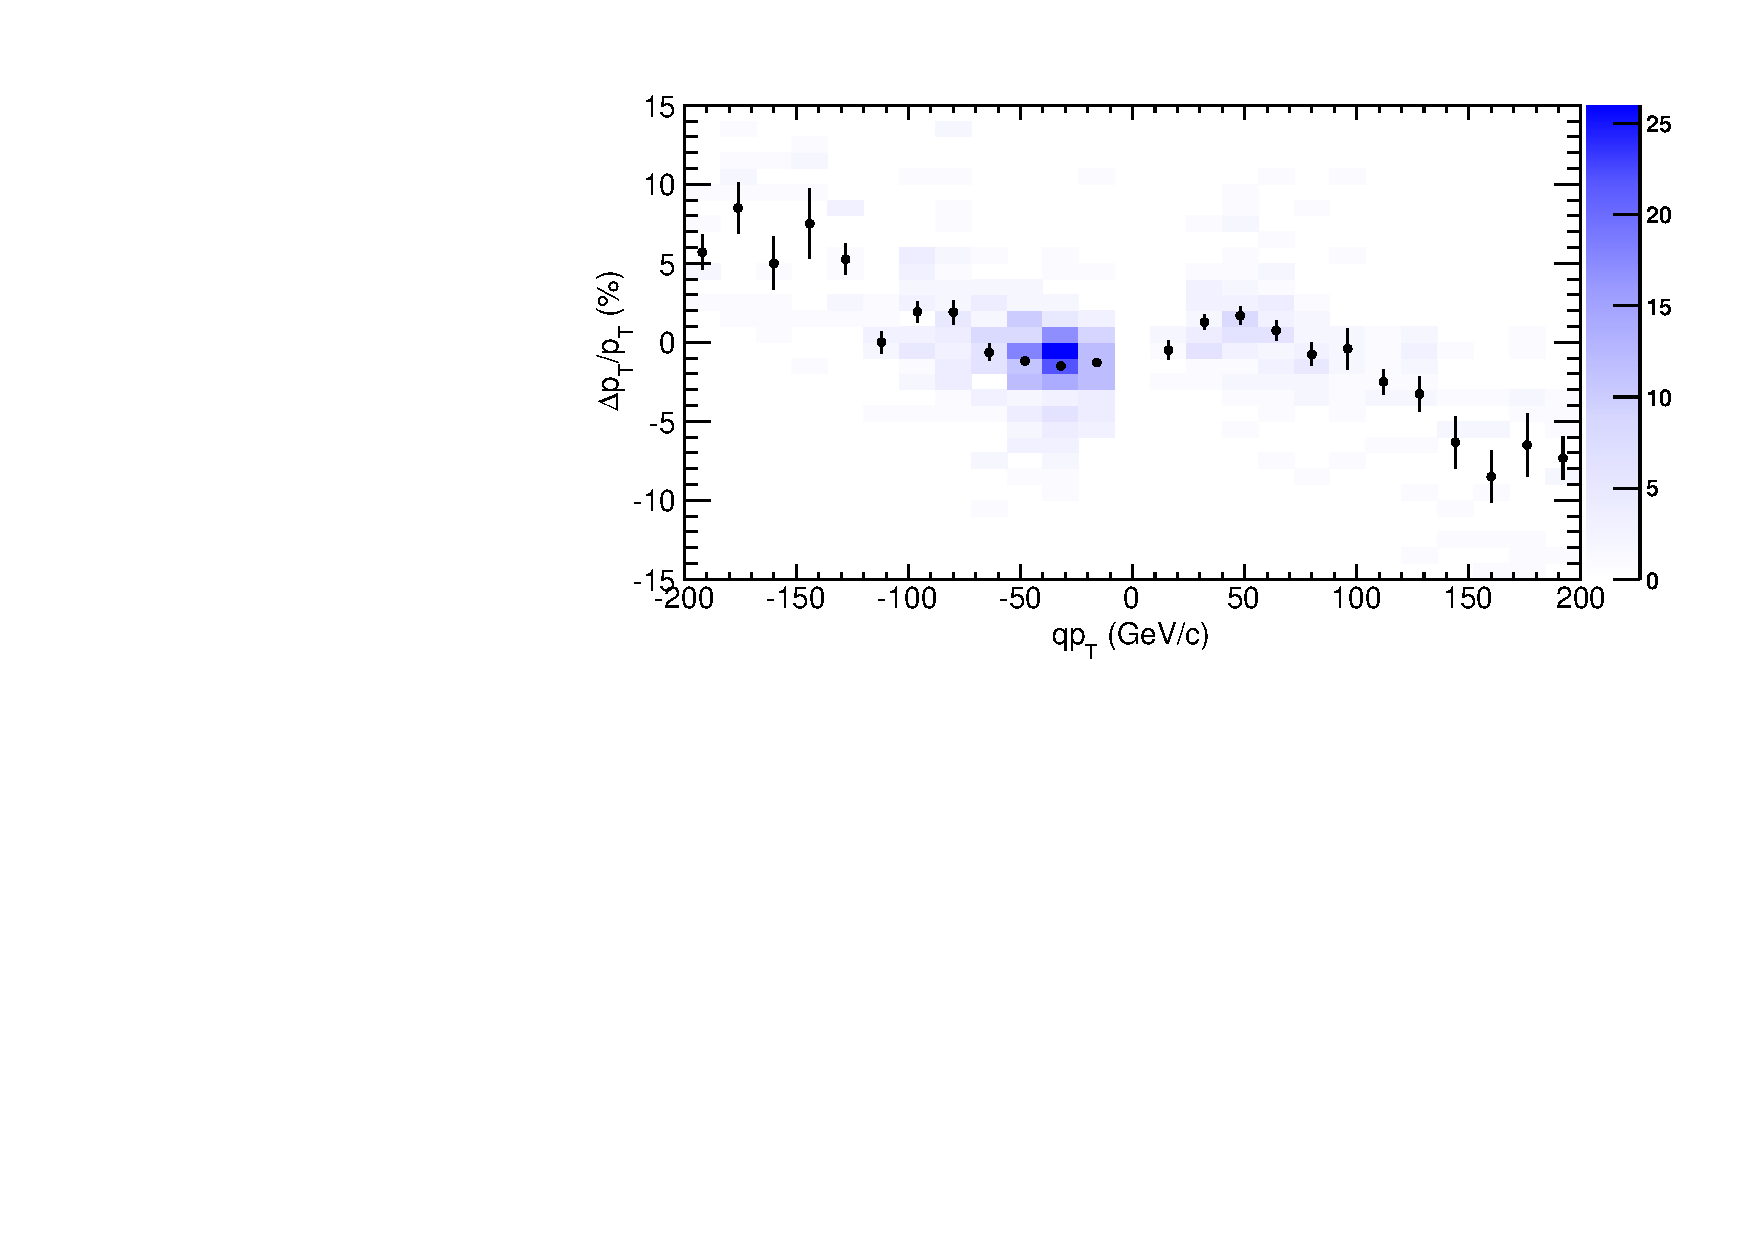
\includegraphics[width=0.8\linewidth]{curvature_errors.pdf}
\end{frame}

\begin{frame}
\frametitle{CSC evens/odds (ME+1/2)}

\begin{itemize}
\item This is the old CSC problem, seen for the first time since last fall
\item The fact that the distribution is symmetric (demonstrated here for the first
  time) rules out magnetic field bias as the cause
\item Not enough statistics to see this on a chamber-by-chamber basis
  (I'll dig further, to see if rebinning might make something visible)
\end{itemize}

\vfill
{\mbox{\hspace{-1 cm}}\begin{minipage}{1.17\linewidth}
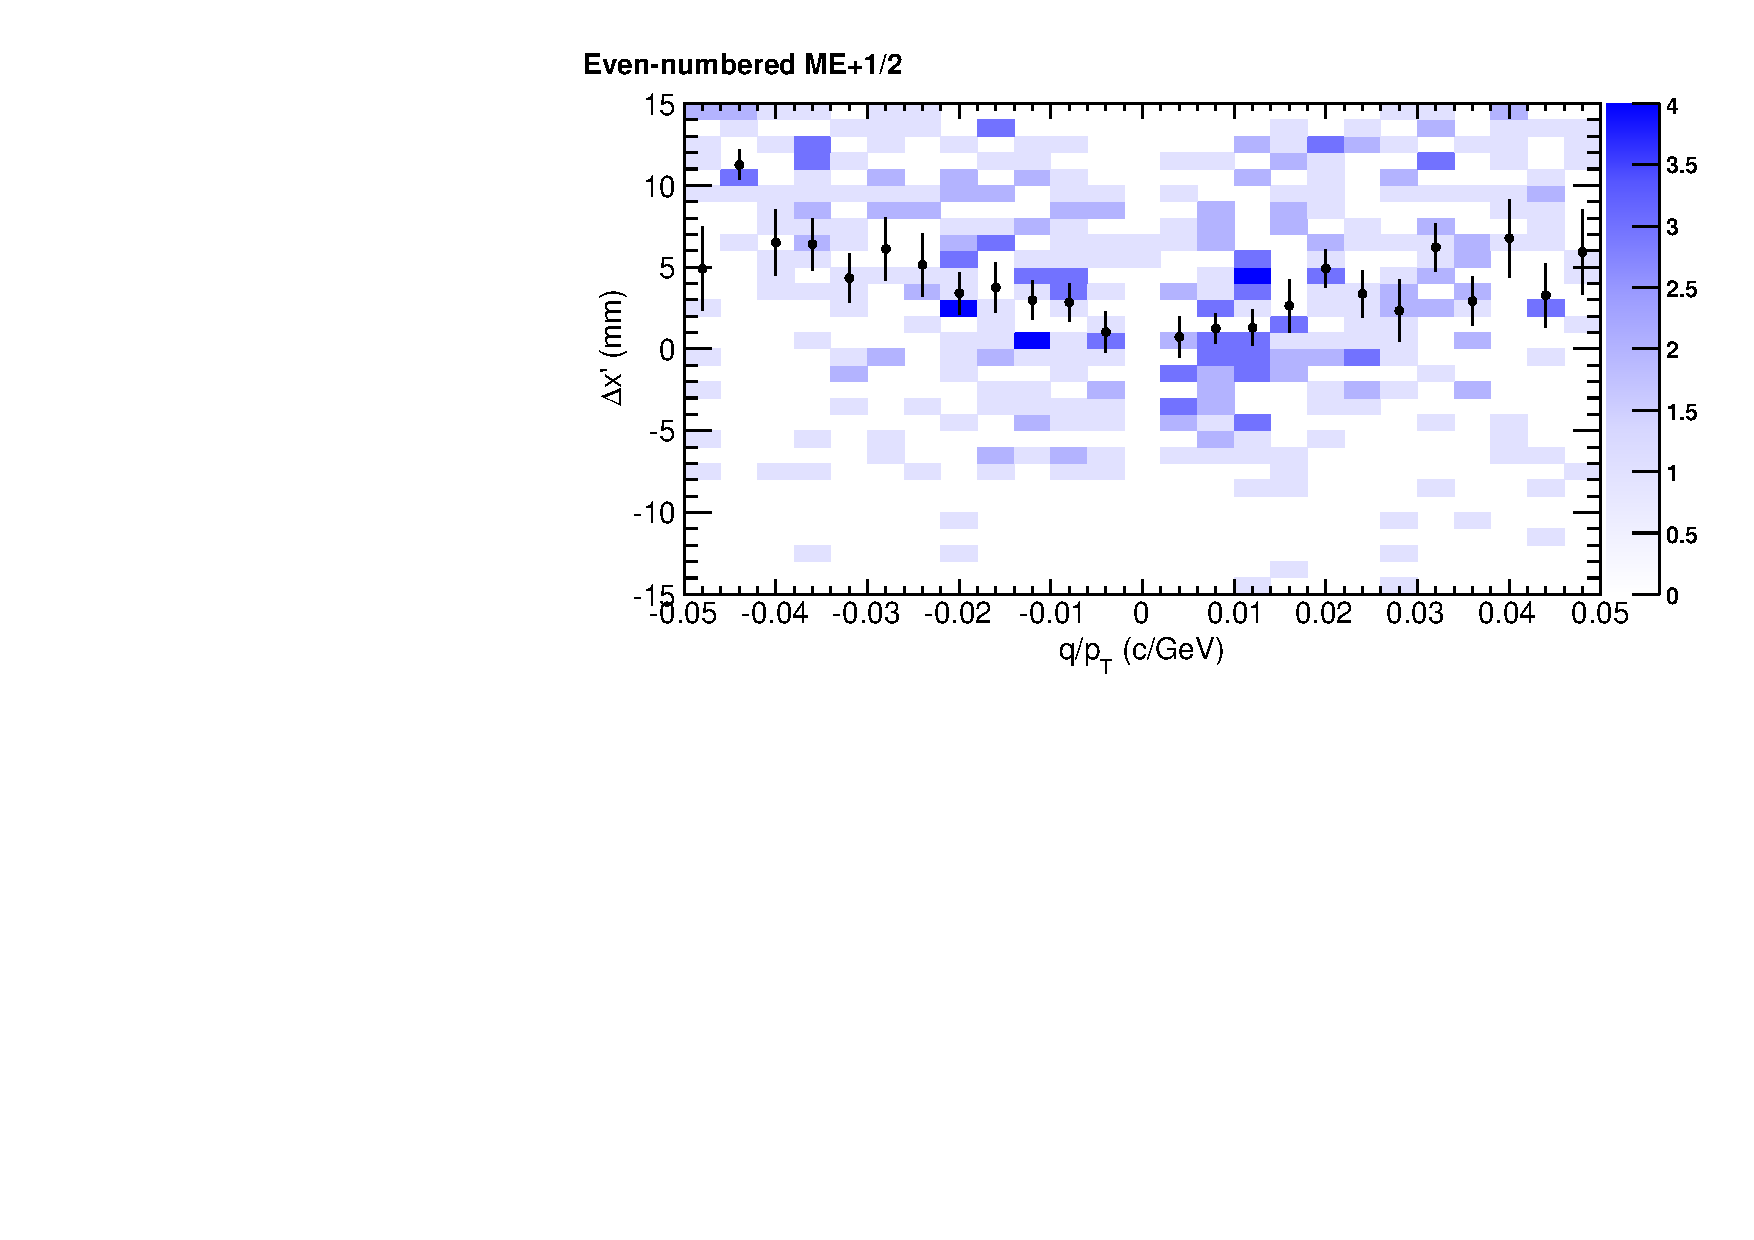
\includegraphics[width=0.5\linewidth]{endcapmep12_evens.pdf}
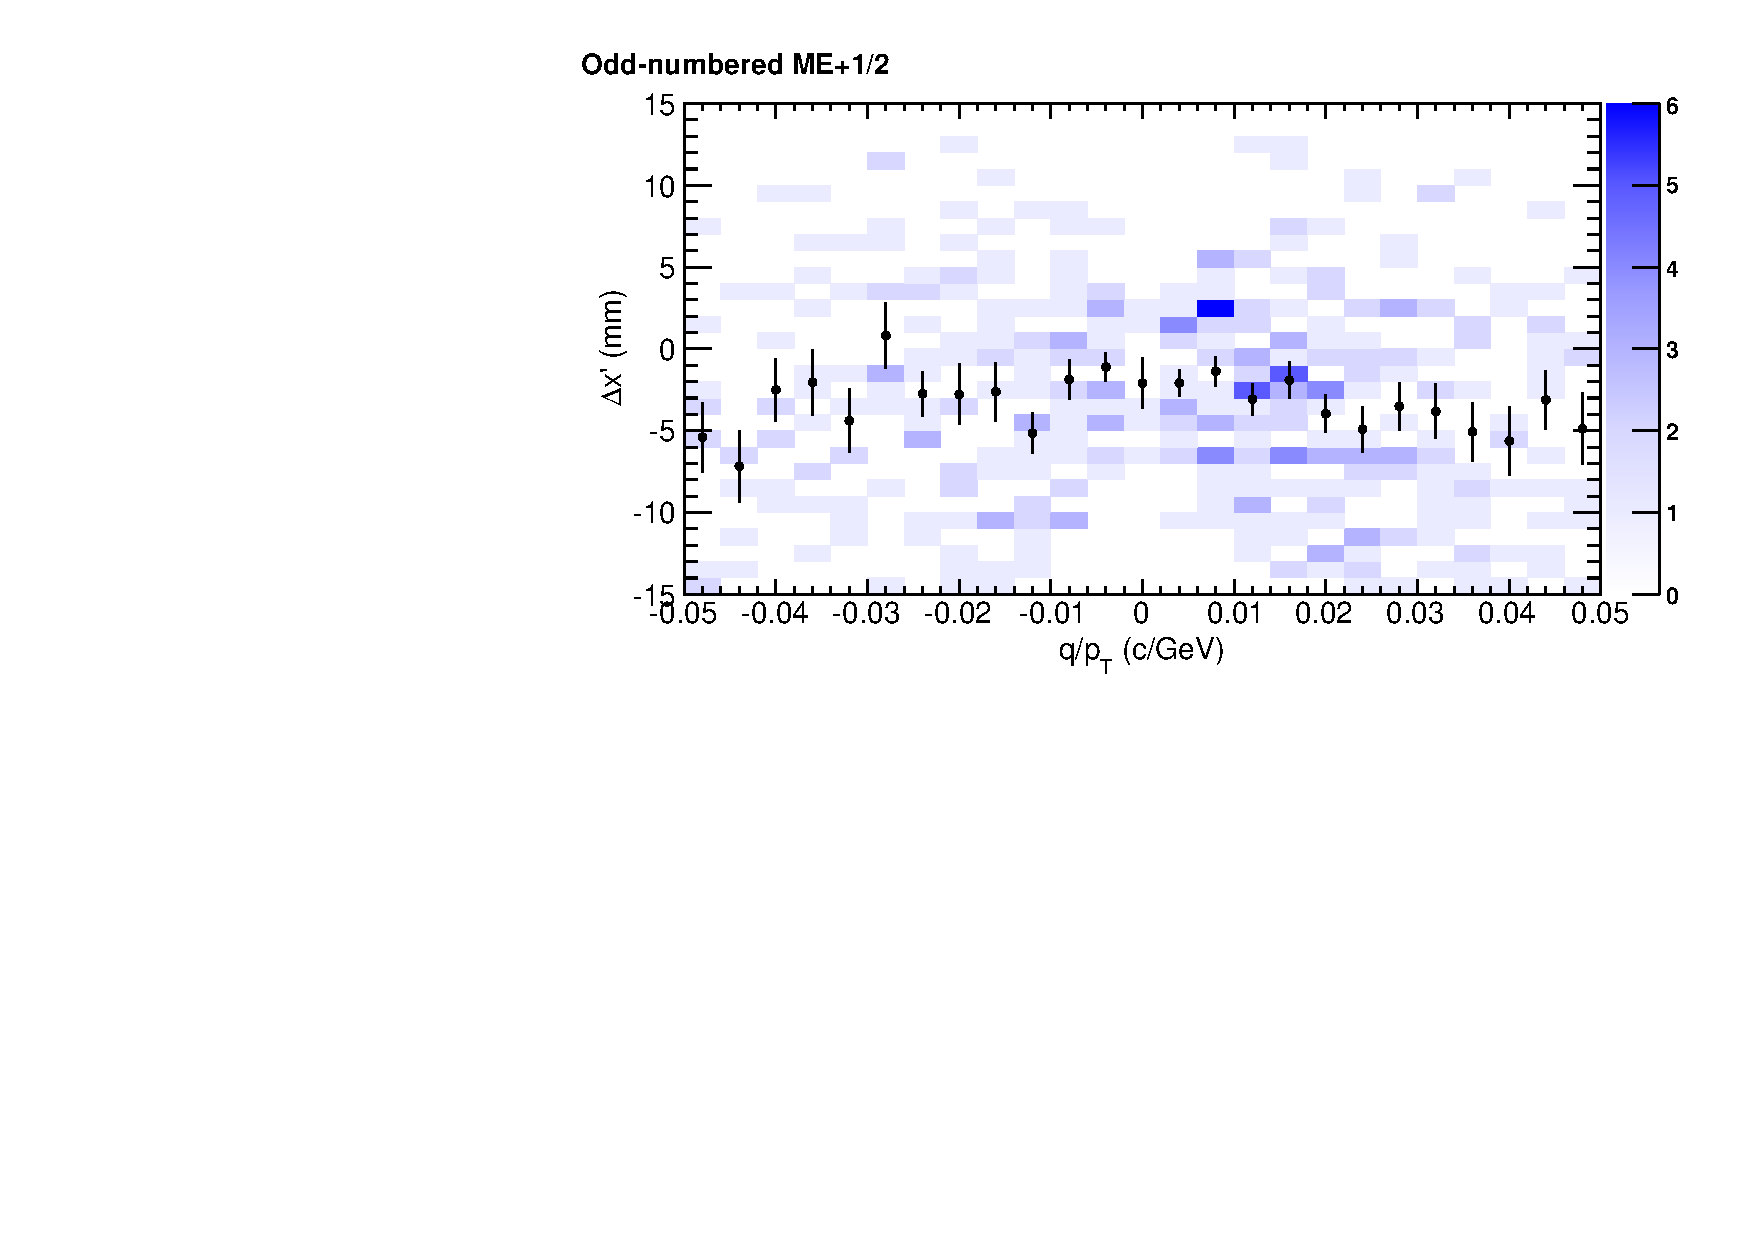
\includegraphics[width=0.5\linewidth]{endcapmep12_odds.pdf}
\end{minipage}}
\end{frame}

\begin{frame}
\frametitle{Summary plot: CRAFT09 tracker}

\begin{itemize}
\item Put the fit results of all barrel chambers on one plot
\item Insensitive to muon misalignment because it's a residuals difference
\item Not much of a pattern vs.\ wheel ($\eta$)
\item Clear pattern vs.\ $\phi$, and it's quadrapole!  (fit to second-order Fourier series)
\end{itemize}

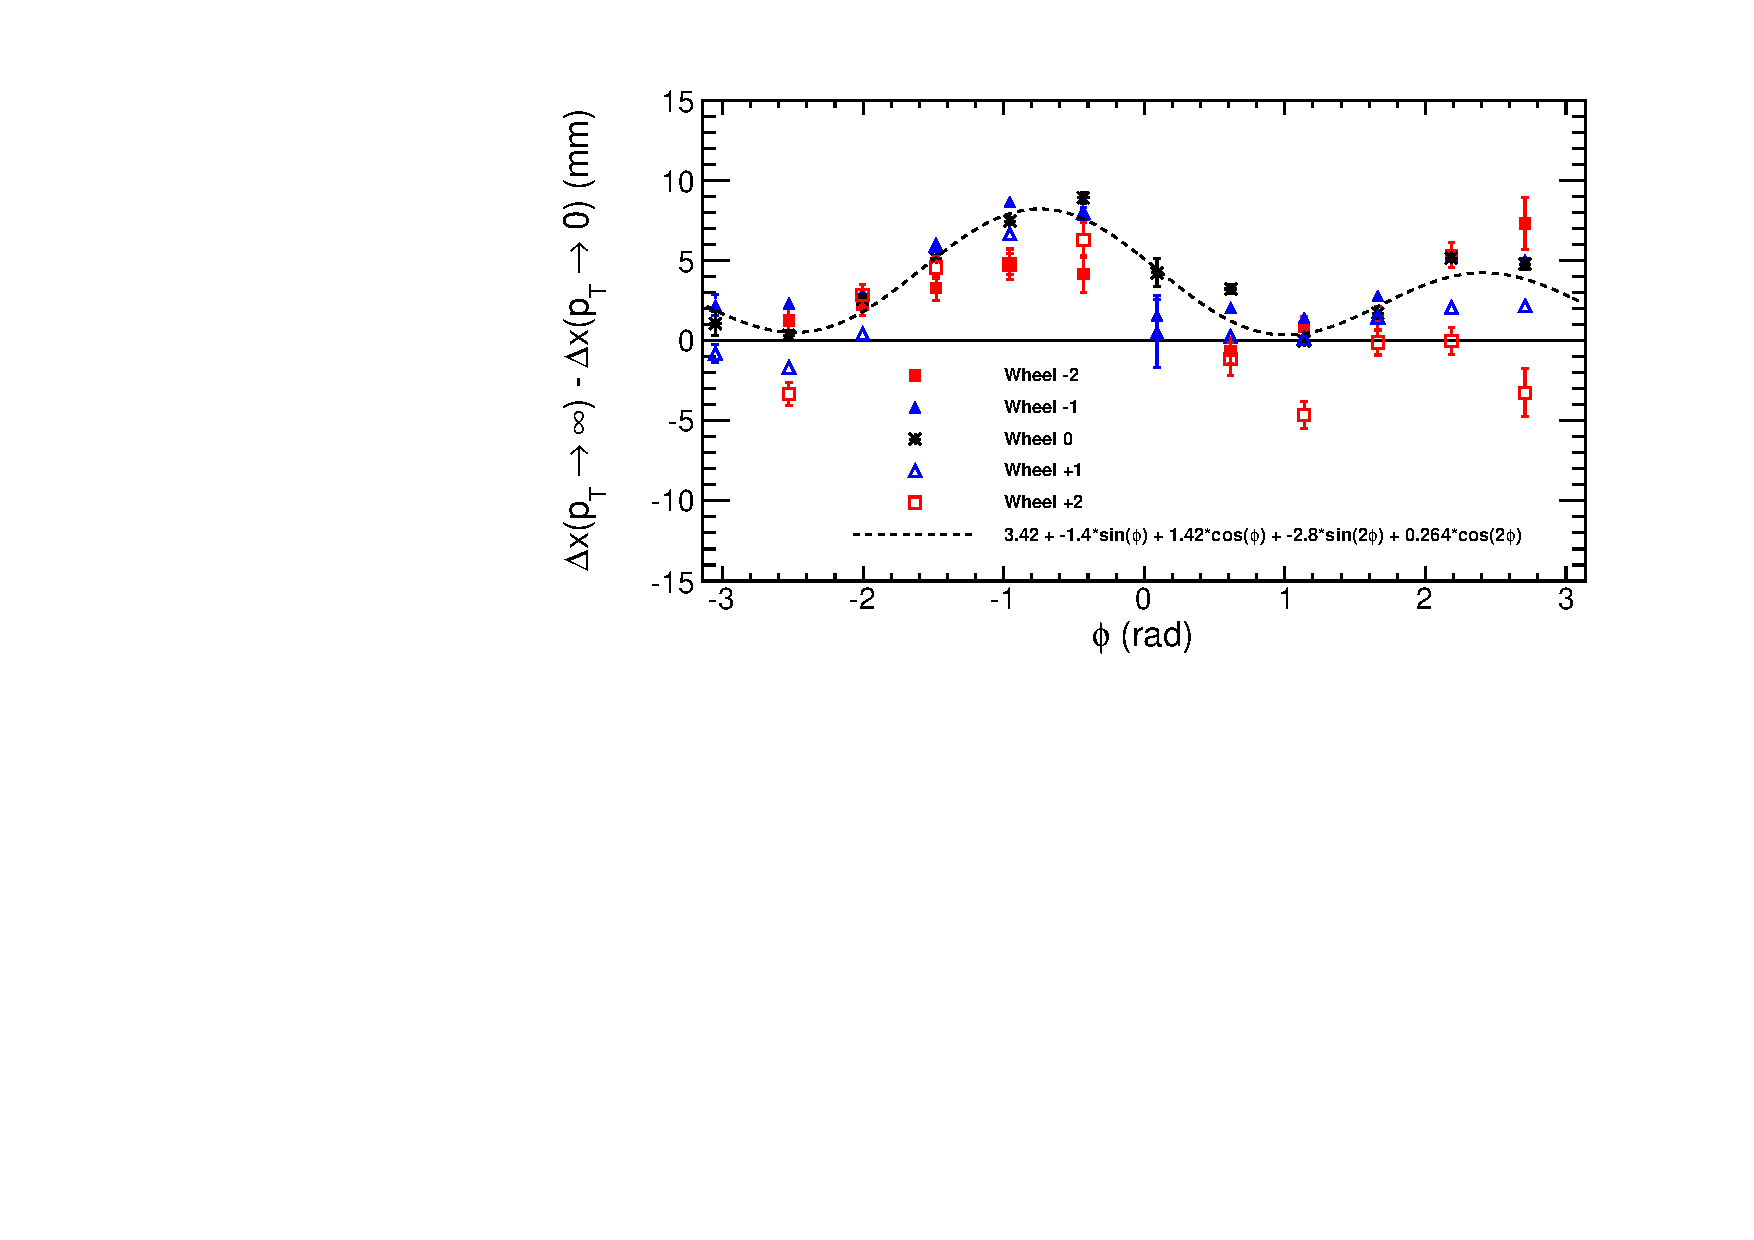
\includegraphics[width=\linewidth]{summary.pdf}
\end{frame}

\begin{frame}
\frametitle{Summary plot: distorted tracker}

\begin{itemize}
\item This is the same thing with the tracker distorted to make the muon chamber at $\phi=-\pi/2$ flat (close to zero in this plot)
\item It differs from the previous slide by an exact $\sin\phi$, which means that we've identified the dipole tracker distortion
\item Now we just need a quadrapole ($\sin 2\phi$) and a monopole ($1$)
\end{itemize}

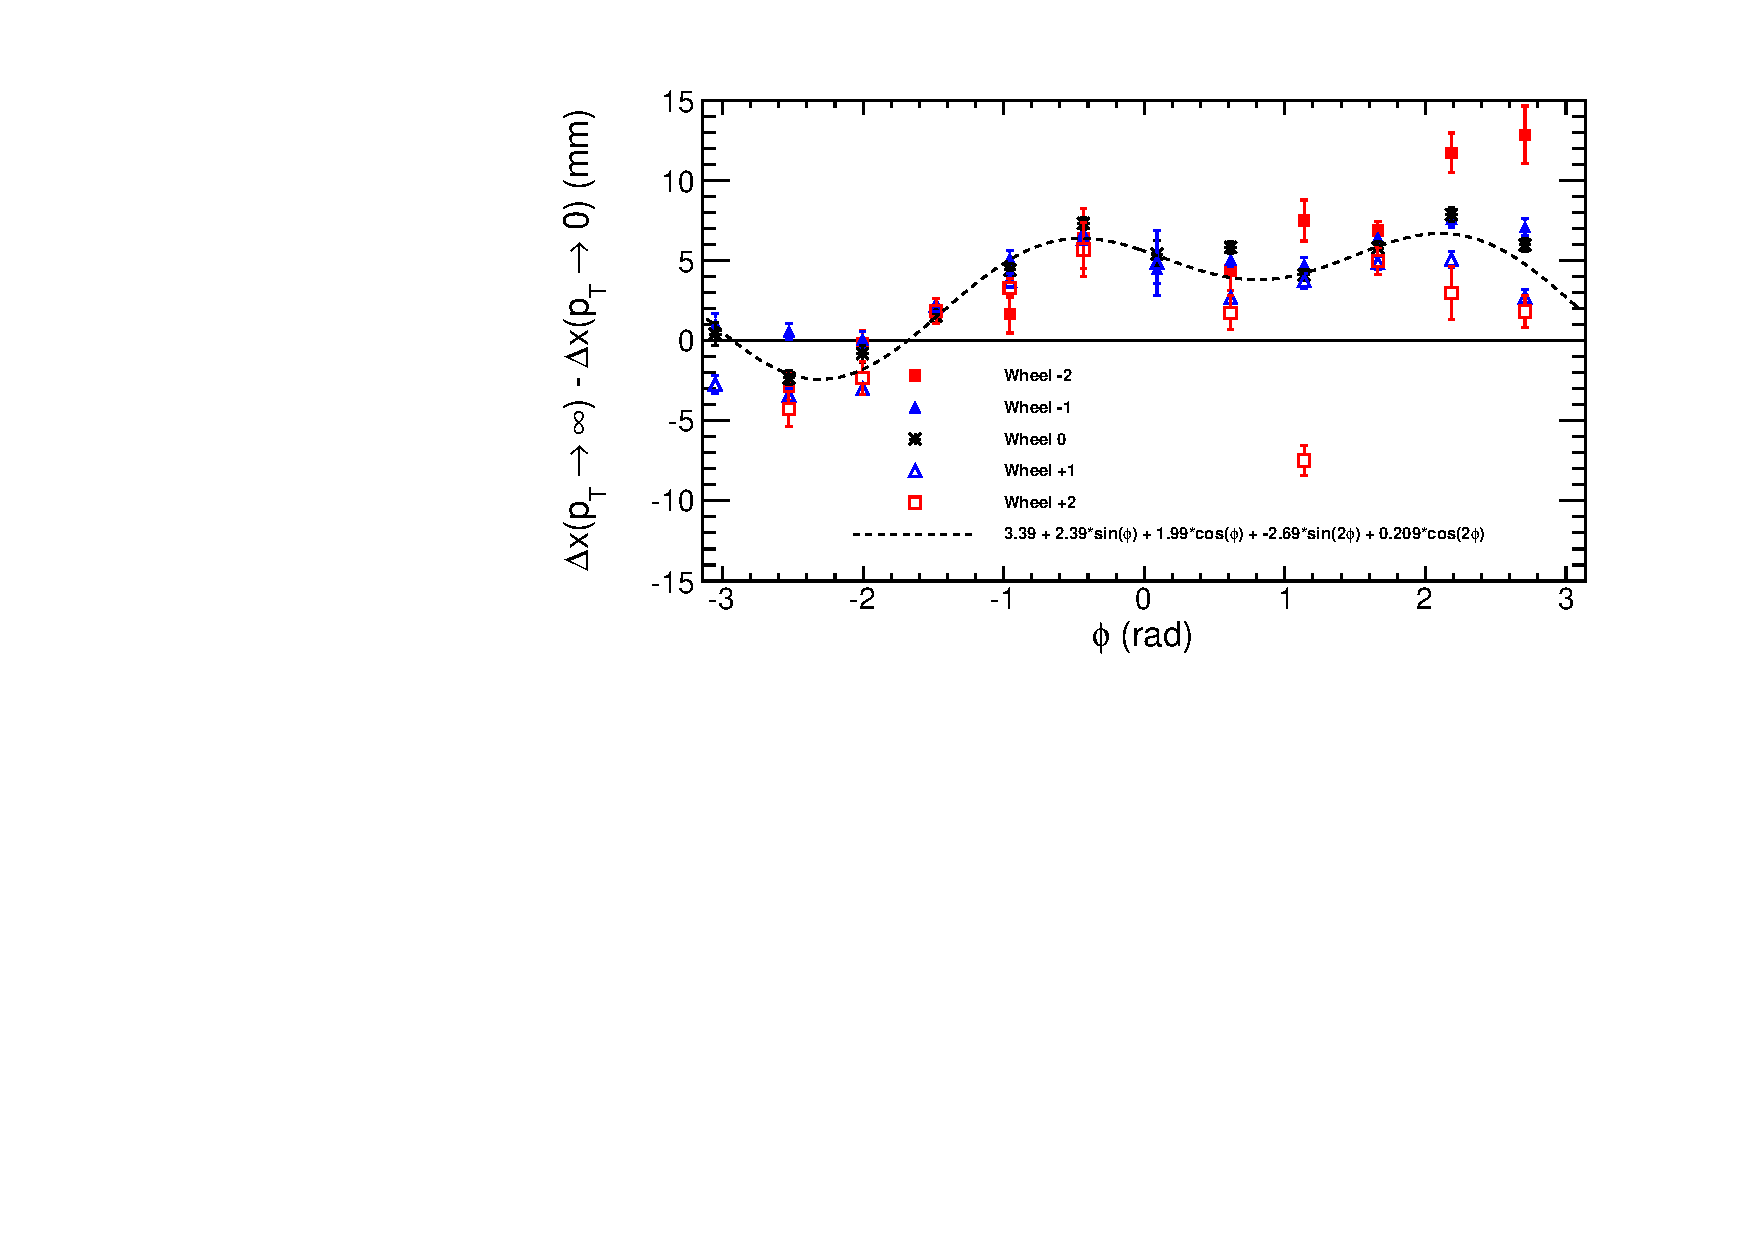
\includegraphics[width=\linewidth]{summary_threekappas.pdf}
\end{frame}

\begin{frame}
\frametitle{Where to go from here}
\begin{itemize}
\item The tracker distortion that Markus found has a perfect $-3.79
  \sin\phi$~mm effect on the summary plot: a to cancel the $-1.40\sin\phi
  + 1.42\cos\phi$~mm effect, we need only apply that distortion with
  0.52$\times$ the magnitude at a $\frac{3}{4}\pi$ angle
\item To cancel the $-2.80 \sin(2\phi) + 0.264 \cos(2\phi)$~mm effect,
  we need to find a distortion which has a quadrapole shape (he thinks
  there are some examples in his thesis to try\ldots), same for the
  3.42~mm monopole effect
\item In the long term, we would need something more automated, but
  doing it by hand now can make the first huge improvement: currently
  all $\mathcal{O}(50\mbox{ GeV/}c)$ and above tracks have the wrong
  momentum by several percent (not just muons)
\item I think we should quickly find and make this correction now, so
  that it doesn't reveal itself as an embarrassing $Z$ peak (ATLAS is
  not likely to have this problem)
\item In muon alignment, we keep monitoring this; in tracker
  alignment, they find a long-term solution
\end{itemize}

\label{numpages}
\end{frame}

\end{document}
